
\subsection{Ikeda's method: from strip theory to semi-empirical formulas}
\label{se:semi-empirical methods}
Since the scale effect of the damping is mainly associated with the skin friction on ship hulls and the friction only contributes very little to a full scale ship's total roll damping, the most reliable way to obtain a ship's roll damping coefficients is to carry out model scale experimental tests. 
While in a ship's early design stage when only limited information is available and flexible to be adjusted, such as the ship's principal dimensions and the basic hull geometry, some semi-empirical methods were also proposed to predict the roll damping \parencite{himeno_prediction_1981}. The most recognize method was developed in a series of research articles \parencite{ikeda_roll_1978,ikeda_eddy_1978,ikeda_roll_1979,ikeda_components_1978,ikeda_velocity_1979}, and it is well-known to be named as Ikeda's method. This method divides the roll damping into five damping components, i.e., the friction component $B_F$, the eddy component $B_E$, the lift component $B_L$, the wave component $B_W$ and the bilge keel component $B_{BK}$, as in the following Eq.(\ref{eq:ikeda}), 

\begin{equation} \label{eq:ikeda}
B = B_F + B_E + B_L + B_W + B_{BK}
\end{equation}

where the wave and eddy components require strip theory based hydrodynamic analysis to get the ship's shape coefficients. The hydrodynamic analysis requires to get a ship's exact hull geometries. It might be time consuming to build the geometry model and perform the strip theory based hydrodynamic analysis. Sometimes, a ship's hull geometry is simply not available for such purposes. 

A simplified Ikeda's method was proposed by \parencite{kawahara_simple_2011} and is instead used in this study to calculate all the damping components including the eddy component $B_E$ and wave component $B_W$. The semi-empirical formulas describe four of the five roll damping components at motion frequency $\omega$ for a given roll amplitude $\phi_a$ at zero ship speed. A speed dependency was introduced by adding a fifth damping term $B_L$ and a speed correction to $B_W$ as described in \parencite{ikeda_velocity_1979} giving a function: 

\begin{equation} \label{eq:simplified_ikeda_equation}
\left( B_{44}, \  B_{F}, \  B_{W}, \  B_{E}, \  B_{BK}, \  B_{L}\right) = \operatorname{Ikeda_{simplified}}\left(L_{pp},beam,C_{b},A_{0},OG,\phi_{a},BK_{L},BK_{B},\omega,T,V\right)
\end{equation}


The hull lift damping is generated when the roll motion is creating a transverse velocity which introduces an angle of attack on the ship hull that generates lift.     
The detailed formulas within $f$ can be referred to \parencite{kawahara_simple_2011}, \parencite{ikeda_velocity_1979} and the actual implementation \parencite{alexandersson_martinlarsalbertrolldecay-estimators_2020}.

%The Simplified Ikeda method \cite{kawahara_simple_2011} has been implemented \cite{alexandersson_martinlarsalbertrolldecay-estimators_2020} with the intention to be used both as a benchmark and maybe also as a sub-component of a new method. The examples from \cite{kawahara_simple_2011} was recalculated to check that the method has been implemented correctly. The authors have been unable to find other ways to validate the implementation, which introduces some uncertainty to the comparisons. The method has been implemented as a function where the total roll damping and its component is calcultated: 



The Ikeda method has been used to calculate the roll damping for a PCTC vessel Faust \parencite{soder_assessment_2019}. For example, Fig. \ref{fig:ikeda_vs_simplified} shows a comparison between roll damping components calculated with the original \emph{Ikeda's method} based on strip theory calculation and the simplified Ikeda's method. The roll damping is under-predicted with the simplified method for this particular case which is expected according to the limitations of this method  \parencite{kawahara_simple_2011}.

\begin{figure}[H]
    \centering
    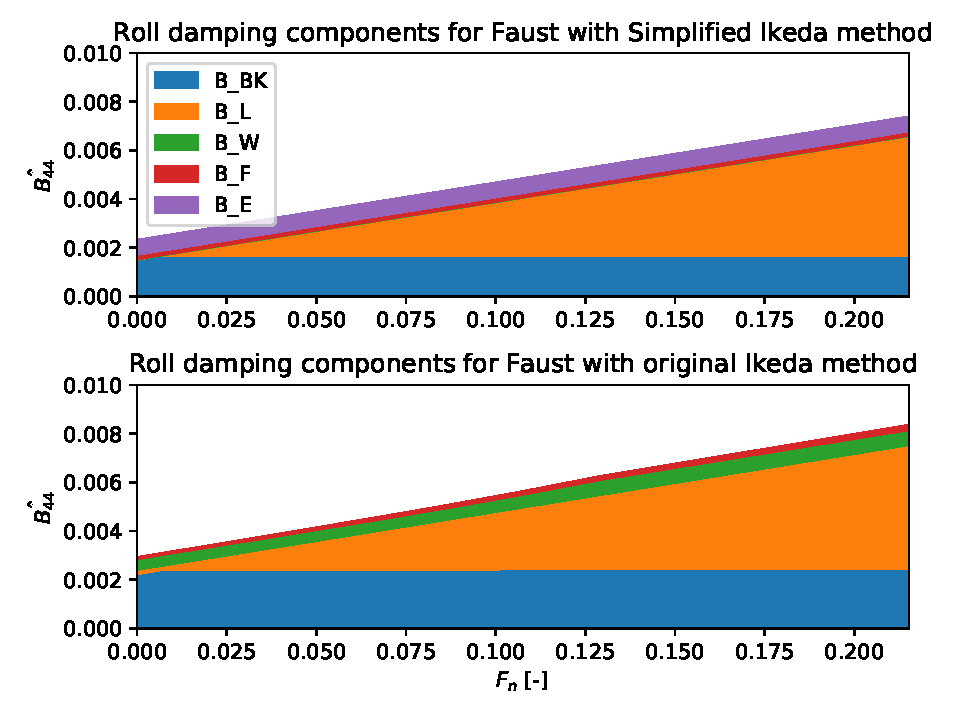
\includegraphics[height=7cm, width=14cm]{figures/ikeda_vs_simplified.pdf}
    \caption{Roll damping components calculated with Ikeda and Simplified Ikeda for PCTC Faust}
    \label{fig:ikeda_vs_simplified}
\end{figure}


